\section{Simulations of SIGGMA Observations}
\label{sec:siggma_simulations}

In this section we describe the RRL measurements from the Survey of Ionized Gas in the Galaxy, Made with the Arecibo Telescope (SIGGMA) \cite{liuSIGGMASURVEYIONIZED2013} and estimate CHORD's ability to detect the HII regions reported by SIGGMA.\\

The SIGGMA survey covers a thin strip of the Galactic plane between Galactic longitudes \(32^\circ \leq \ell \leq 70^\circ\) and Galactic latitudes \(|b| \leq 1.5^\circ\) with a frequency range of 1225 MHz to 1525 MHz. A plot of the SIGGMA data showing the overlap with CHORD is shown in Figure \ref{fig:siggma_with_chord_coverage}. The survey averages the intensity profile of 12 RRLs (H163\(\alpha\) to H174\(\alpha\)) and covers a velocity range of \(\pm 300 \km \s^{-1}\) with a \(5.1 \km \s^{-1}\) channel resolution. An inner-Galaxy data release \cite{liuSurveyIonizedGas2019} provides measurements of 244 known HII regions and an additional 79 candidate regions\footnote{Data available at \url{https://cdsarc.cds.unistra.fr/viz-bin/cat/J/ApJS/240/14t}}, of which 14 and 12, respectively, are within the CHORD survey range. A subset of these is provided in Table \ref{tab:siggma_candidates}.
% \begin{figure}[h]
%     \centering
%     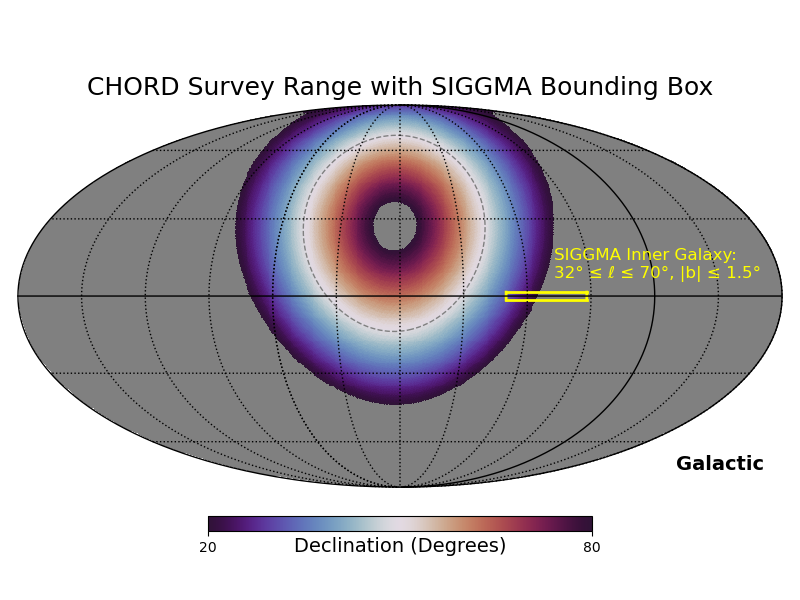
\includegraphics[width=0.5\textwidth]{plots/siggma/siggma_range_map.png}
%     \caption{The SIGGMA survey range (yellow box) overlaid on the CHORD survey range, showing only partial overlap between the two.}
%     \label{fig:siggma_range_map}
% \end{figure}

\begin{figure}[h]
    \centering
    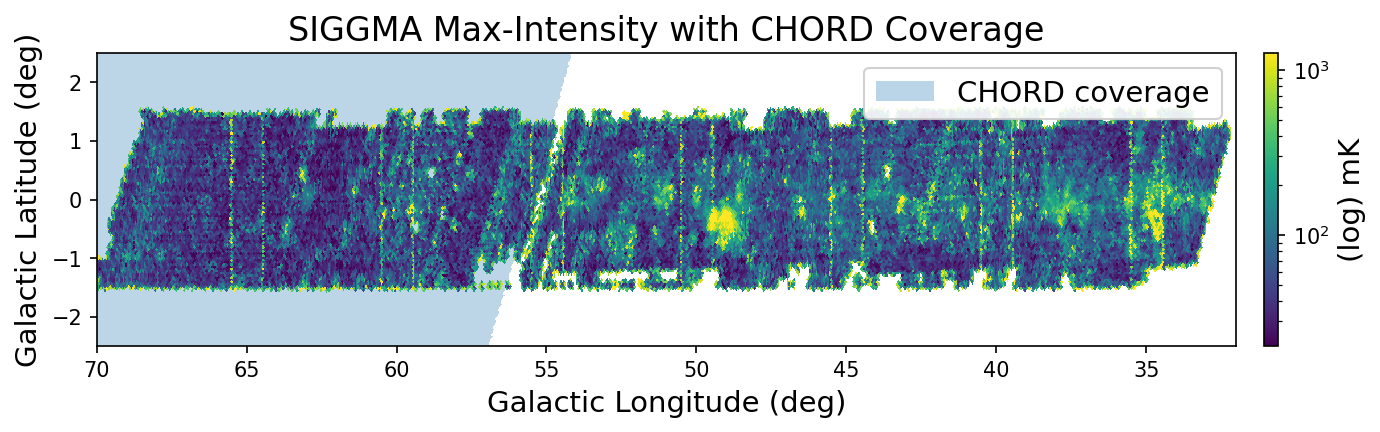
\includegraphics[width=1\textwidth]{thesis/plots/siggma/siggma_with_chord_coverage.png}
    \caption{The SIGGMA data products showing peak intensity per pixel, the area covered by CHORD is highlighted in blue.}
    \label{fig:siggma_with_chord_coverage}
\end{figure}
\begin{figure}[h]
    \centering
    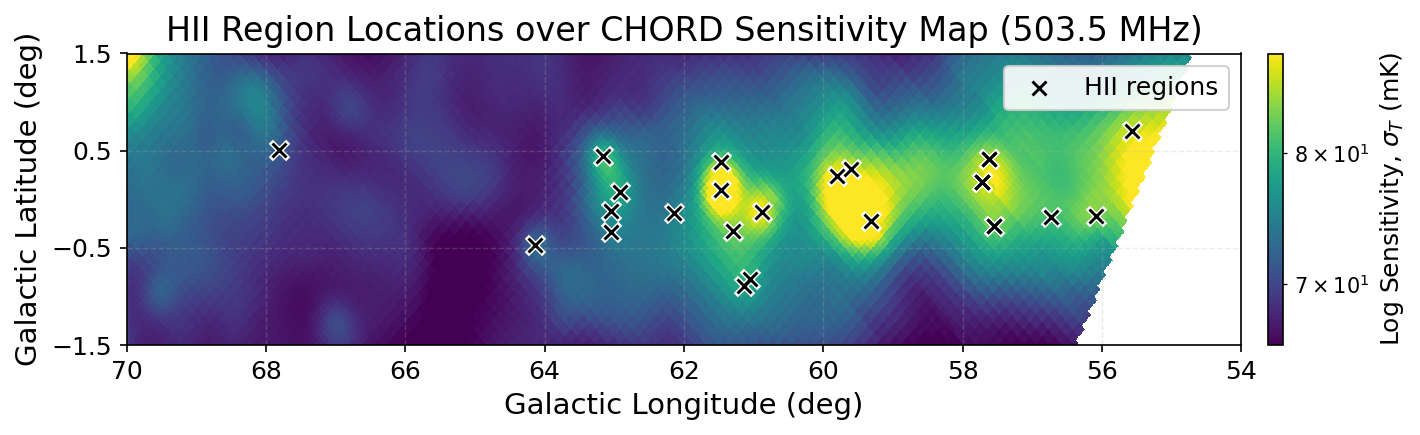
\includegraphics[width=1\linewidth]{thesis/plots/siggma/hii_regions_over_chord_sensitivity.png}
    \caption{HII regions detected by SIGGMA plotted over the CHORD sensitivity map at 503 MHz, showing that most HII regions are in places with high background noise.}
    \label{fig:hii_regions_over_chord_sensitivity}
\end{figure}

\begin{table}[H]
    \centering
    \begin{tabular}{l c c c c c}
        \toprule
        Order & Name  & Peak [mK] & FWHM [km/s] & SNR & Type \\
        \midrule
        1 & G063.164+00.449 & $694.5 \pm 40.6$ & $16.5 \pm 1.1$ & 16.9 & Known \\
        2 & G061.473+00.094 & $348.6 \pm 26.9$ & $30.1 \pm 2.7$ & 12.8 & Known \\
        3 & G059.796+00.241 & $124.5 \pm 11.4$ & $33.2 \pm 3.5$ & 10.7 & Known \\
        $\vdots$ & $\vdots$ & $\vdots$ & $\vdots$ & $\vdots$ & $\vdots$ \\
        25 & G057.715+00.173 & $17.1 \pm 1.7$ & $68.7 \pm 11.3$ & 16.6 & Candidate \\
        26 & G062.142-00.144 & $16.8 \pm 2.6$ & $63.9 \pm 11.7$ & 6.2 & Candidate \\
        \bottomrule
    \end{tabular}
    \caption{A subset of the HII region results reported by SIGGMA which are within the CHORD coverage, ordered from highest to lowest peak line strength, a full table is available in appendix \ref{sec:siggma_appendix}.}
    \label{tab:siggma_candidates}
\end{table}

The 12 stacked lines have an average frequency of 1375 MHz, so we define the peak line strength as the measurement at this reference frequency, \(T_{L}(1375\,\MHz)\). We can then obtain the peak line strength for each line in the CHORD frequency range by scaling from this reference frequency,
\begin{equation}
    T_{L}(\nu) = T_{L}(1375\,\MHz) \frac{1375 \MHz}{\nu}.
\end{equation}

The single-day per-line SNR of each of the 26 HII regions is computed using the CHORD sensitivity at the given HII region location and is shown in Figure \ref{fig:SNR_per_SIGGMA_line}. SNR is maximized between 500 and 600 MHz, which is expected for observations along the Galactic plane. The lowest single-day per-line SNR is around 0.5, while the highest is 24. The two very bright HII regions `G063.164+00.449' and `G061.473+00.094' are significant outliers, with SNRs of 24 and 10, respectively, and are omitted from Figure \ref{fig:SNR_per_SIGGMA_line}.

\begin{figure}[H]
    \centering
    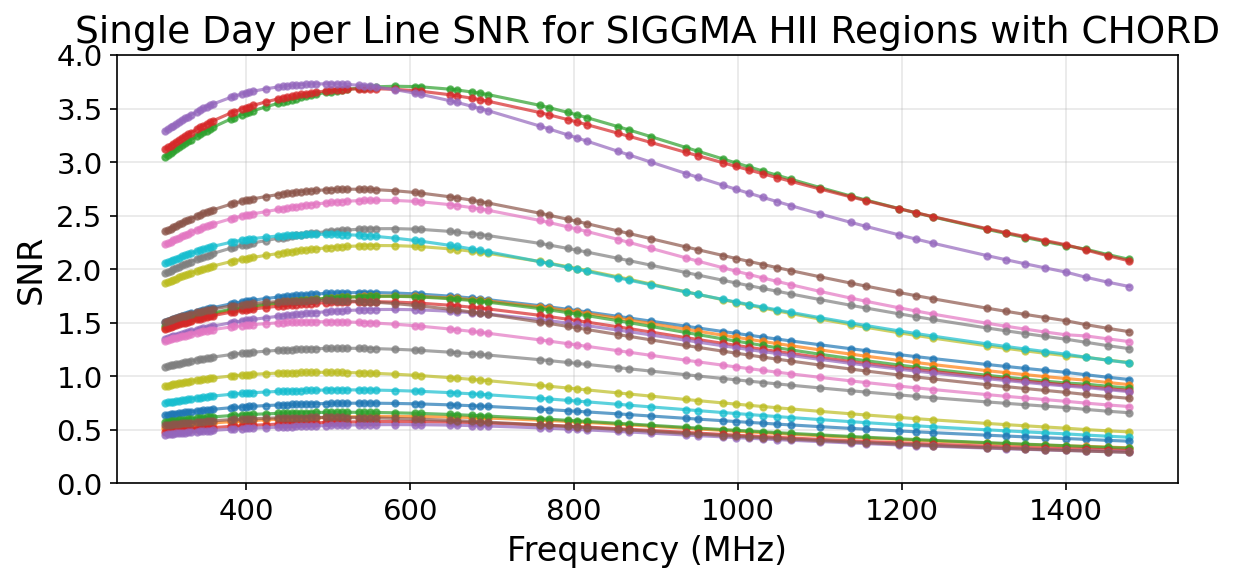
\includegraphics[width=1\linewidth]{thesis/plots/siggma/SNR_per_SIGGMA_line.png}
    \caption{Single-day per-line SNR for 24 HII regions within the CHORD coverage, excluding the two very bright outliers, showing that SNR peaks between 500 and 600 MHz and is in the range 0.5 to 3.7.}
    \label{fig:SNR_per_SIGGMA_line}
\end{figure}

We simulated the line-stacking process described in section \ref{sec:line_stacking} for the top 1, 15 and 60 lines of each HII region. The resultant SNR predictions for one observing day are shown in Table \ref{tab:siggma_stacked_snr}. The lowest single day SNR with 60 stacked lines is \(3.93 \pm 0.39\) which demonstrates that each region should be easily detectable by CHORD. Furthermore, each observing day is an independent sample so SNR increases in proportion to the square root of the number of observing days. A true survey will observe each region between 9 and 36 days, meaning SNR is expected to increase by a factor of 3 to 6.

\begin{table}[H]
    \centering
    \begin{tabular}{l c c c c}
        \toprule
        Order & Name  & SNR top 1 & SNR top 15 & SNR top 60 \\
        \midrule
        1 & G063.164+00.449 & $23.5 \pm 1.4$ & $90.98 \pm 5.32$ & $171.54 \pm 10.03$ \\
        2 & G061.473+00.094 & $9.72 \pm 0.75$ & $37.47 \pm 2.89$ & $70.73 \pm 5.46$ \\
        3 & G059.796+00.241 & $3.71 \pm 0.34$ & $14.26 \pm 1.31$ & $26.71 \pm 2.45$ \\
        $\vdots$ & $\vdots$ & $\vdots$ & $\vdots$ & $\vdots$ \\
        25 & G057.715+00.173 & $0.55 \pm 0.05$ & $2.10 \pm 0.21$ & $3.93 \pm 0.39$ \\
        26 & G062.142-00.144 & $0.61 \pm 0.09$ & $2.37 \pm 0.37$ & $4.45 \pm 0.69$ \\
        \bottomrule
    \end{tabular}
    \caption{SNR for CHORD observations of SIGGMA HII regions using one observing day, showing SNR from stacking the top 1, 15 and 60 lines, a full results table is in appendix \ref{sec:siggma_appendix}.}
    \label{tab:siggma_stacked_snr}
\end{table}